\documentclass[12pt,letterpaper]{article}
\usepackage[margin=1in]{geometry}
\usepackage{fancyhdr}
\usepackage[utf8]{inputenc}
\usepackage{palatino}
\usepackage{microtype}
\usepackage{hyperref}
\usepackage{graphicx}
\usepackage{lastpage}
\usepackage[hang,small,margin=1in]{caption}
\usepackage{titlesec}

\renewcommand{\headrulewidth}{0pt}
\fancyfoot{}
\fancyfoot[C]{\sffamily Page \thepage\ of \pageref{LastPage}}
\pagestyle{fancy}

\titleformat{\section}{\bfseries\MakeUppercase}{\arabic{\thesection}}{1em}{}
\titleformat{\subsection}{\bfseries}{\arabic{\thesection}.\arabic{\thesubsection}}{1em}{}
\titleformat{\subsubsection}{\itshape}{\arabic{\thesection}.\arabic{\thesubsection}.\arabic{\thesubsubsection}}{1em}{}

\setlength{\parindent}{0cm}
\setlength{\parskip}{1em}

\captionsetup[figure]{labelfont=it, font=it}
\captionsetup[table]{labelfont={it,sc}, font={it,sc}}

\hypersetup{colorlinks, linkcolor = black, citecolor = black, urlcolor = black}
\urlstyle{same}



\begin{document}

\fancyfoot{}
\begin{center}
    \hfill \\
    \vspace{4in}
    {\bf\Huge CS457 Project \#7 \\}
    \vspace{2in}
    {\Large Soo-Hyun Yoo \\ March 4, 2015}
\end{center}

\newpage
\fancyfoot[C]{\sffamily Page \thepage\ of \pageref{LastPage}}

\section*{Source Files}

\begin{itemize}
    \item p7.glib
    \item p7.vert
    \item p7.frag
\end{itemize}


\section*{Explanation}

\subsection*{p7.glib}

We put ourselves in orthographic mode, place the eye at positive Z, and point
the camera at the origin with positive Y as the up vector.

We declare the vertex and fragment files to be used as well as some variables
to display in sliders and checkboxes. We draw a ground and a background sphere
and import the bunny as our object.

\subsection*{p7.vert}

We output some position vectors for lighting in the fragment shader.

\subsection*{p7.frag}

We declare the input vectors and uniform variables.

After setting the color, we generate some fog with a small amount of noise that
varies with time. We use the atan function to cause the fog to step off more
obviously and mix the object color with the fog using {\tt fogDensity} as the
mix ratio.

\newpage
\section*{Results}

\begin{figure}[!h]
    \centering
    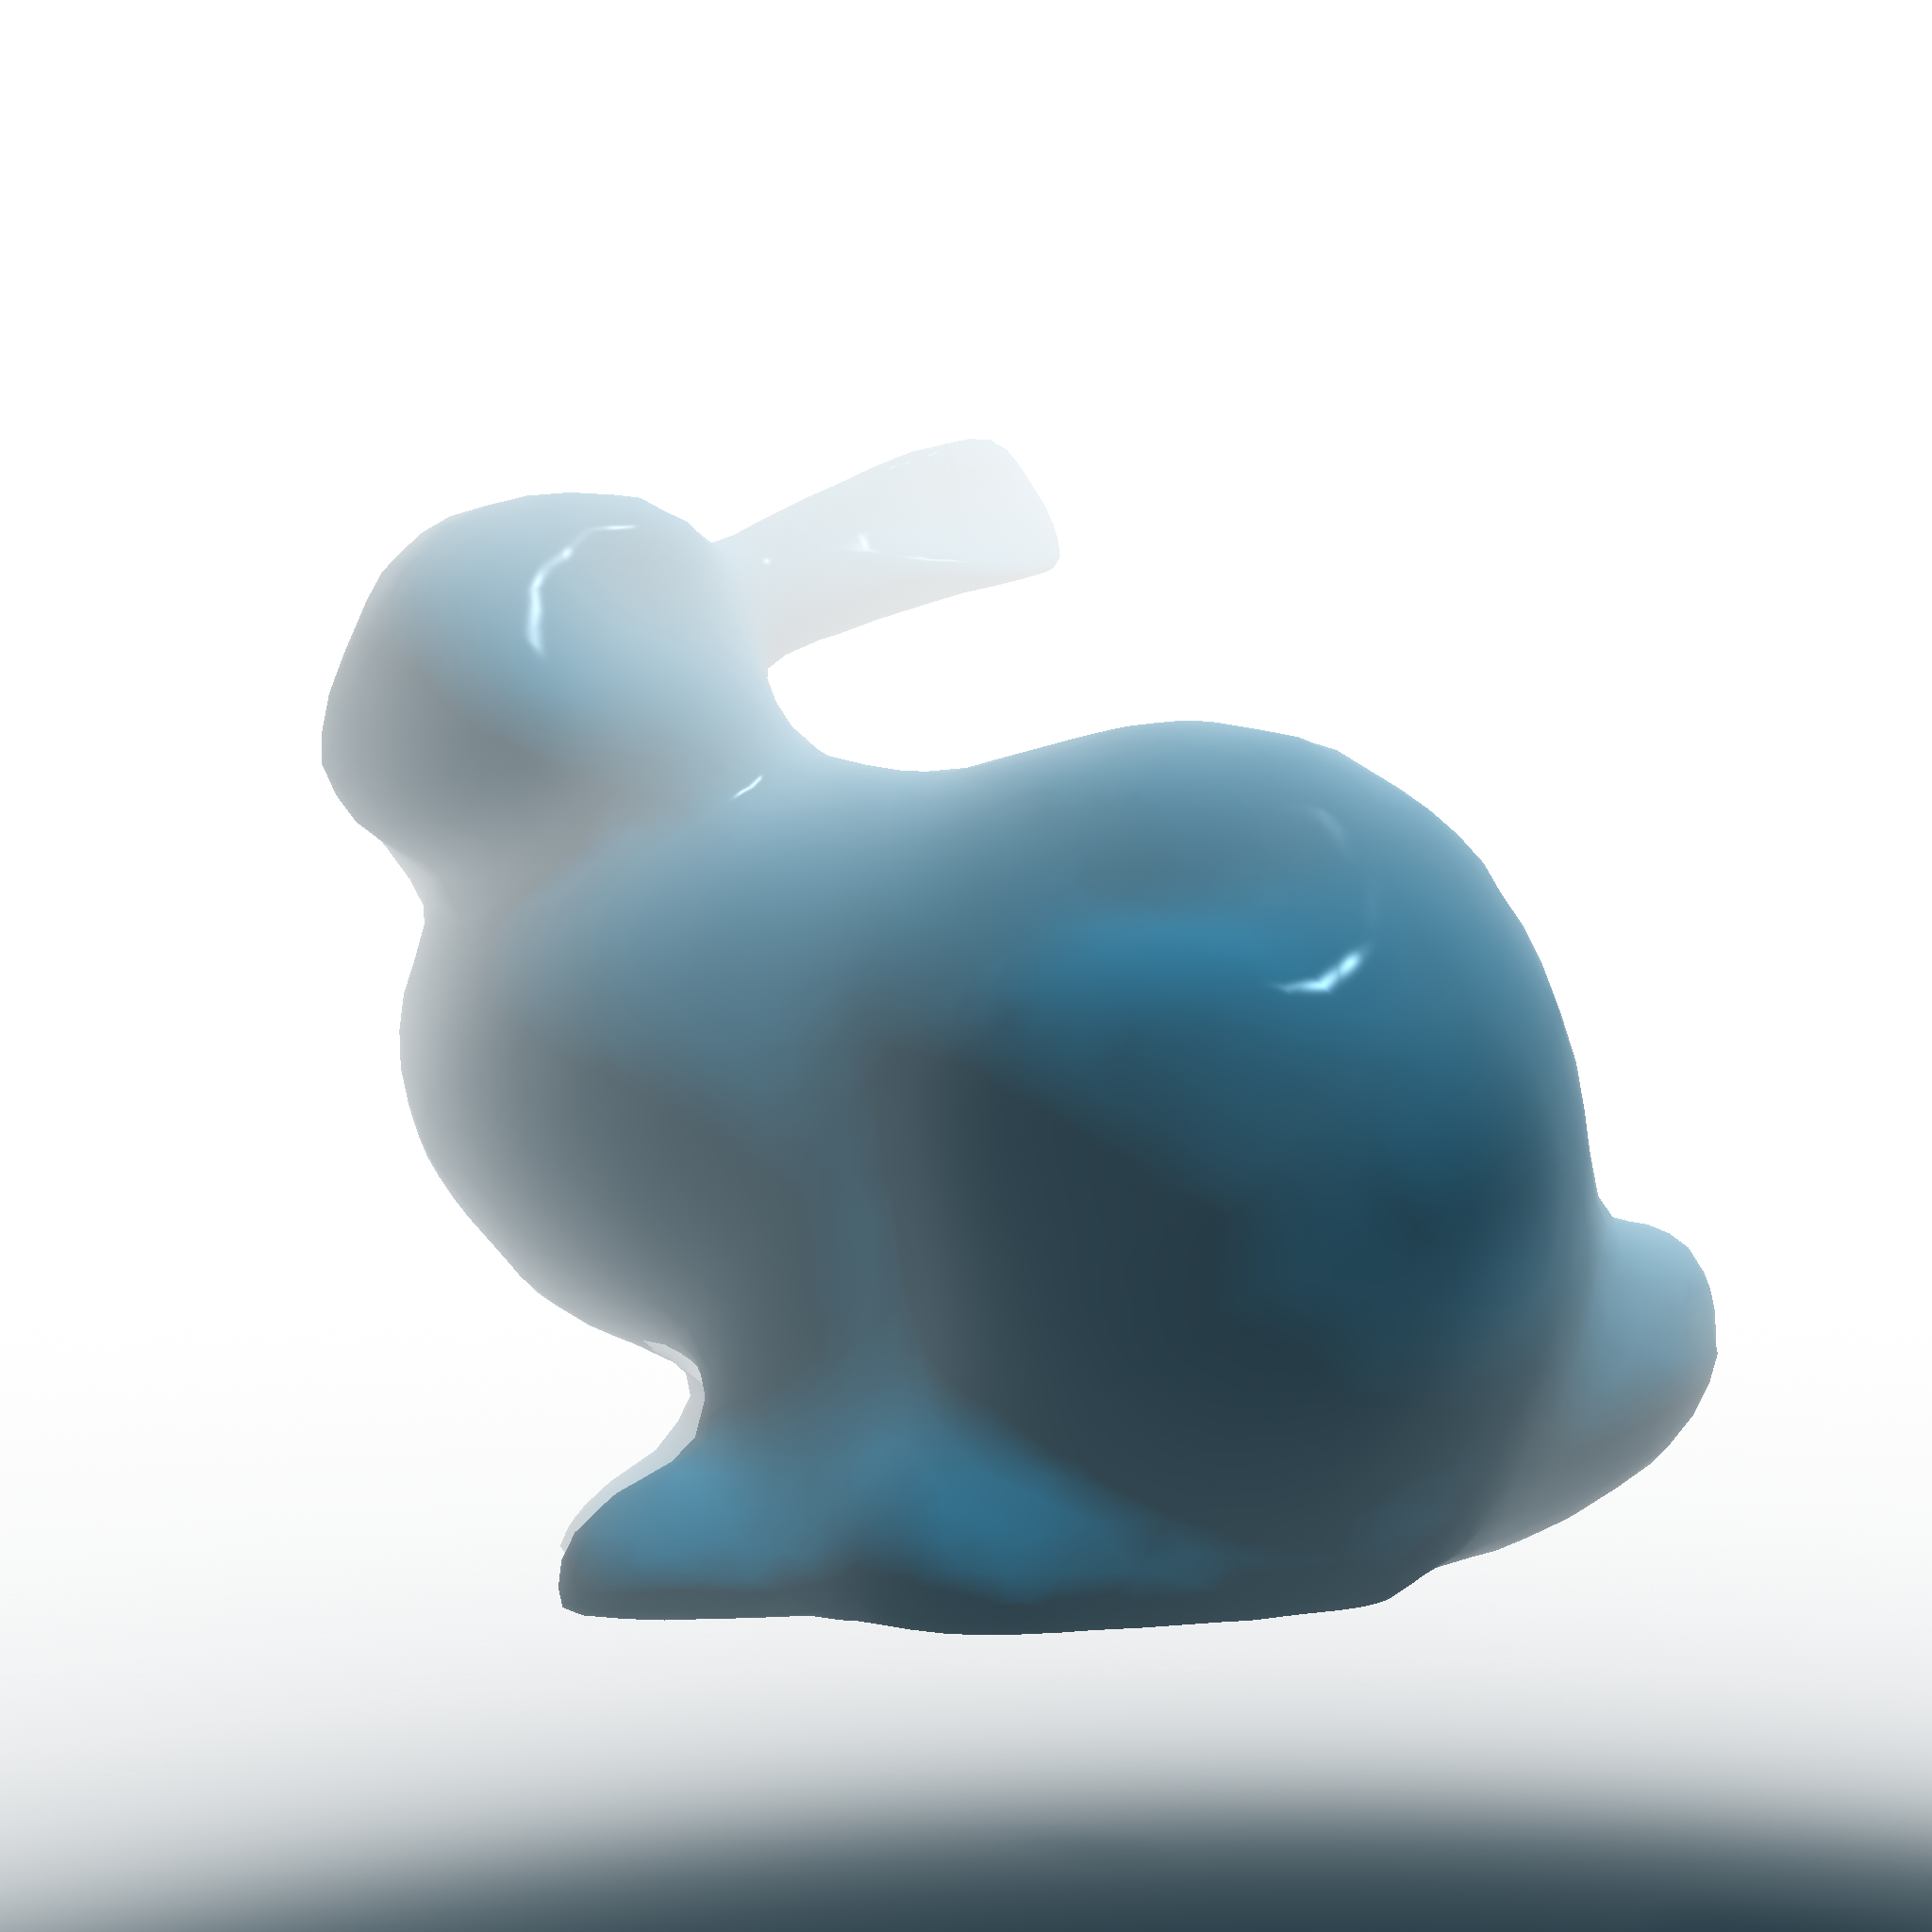
\includegraphics[width=1.0\textwidth]{img/fogbunny.png}
    \caption{Bunny in fog.}
\end{figure}

\end{document}
